\chapter{Présentation de l’application et de ses fonctionnalités}

L’application que nous devons enrichir á été développé par Hanaë Rateau dans le cadre de son doctorat au sein de l’équipe MINT. Cette application consiste à traquer, via la Kinect, un ou plusieurs utilisateurs et leurs permettre de créer des espaces d’interactions pour pouvoir contrôler à distance la souris de l’ordinateur sur plusieurs écrans.

\section{Espace d’interaction virtuel}

L’espace d’interaction virtuel, comme décrit dans l'article de \textit{Rateau et al.} \cite{rateau:hal-00851935},  est une notion qui consiste à réserver une partie de l’espace de l’utilisateur pour interagir. Cet espace d’interaction peut être de différentes dimensions comme une courbe, une surface plane ou un volume.  Dans l’application, cet espace virtuel est utilisé pour contrôler le curseur de la souris sur plusieurs écrans (en mode bureau étendu). L’utilisateur peut changer d’écran en faisant un geste partant de l’espace vers l’écran concerné. Pour l’instant, il n’est possible de travailler que sur 2 écrans positionnés à des endroits fixes. Pour créer un espace d’interaction virtuel, l’utilisateur doit dessiner un carré dans l’espace. 
	 
\begin{figure}[!ht]
	\center	
	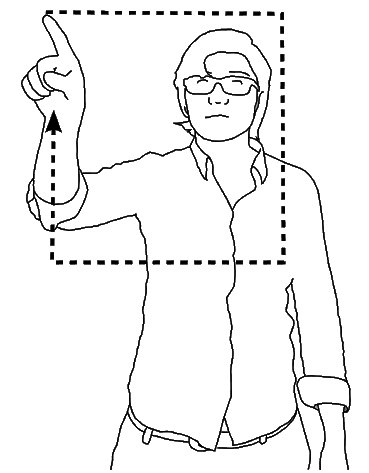
\includegraphics[scale=0.2]{image/create.png}
	\caption{Création de l'espace d'interaction virtuel}
\end{figure}

Cet espace virtuel ne peut pas être déplacé par les utilisateurs mais peut être supprimé par un mouvement rapide ayant pour représentation de pousser l’espace virtuel.

\begin{figure}[!ht]
	\center	
	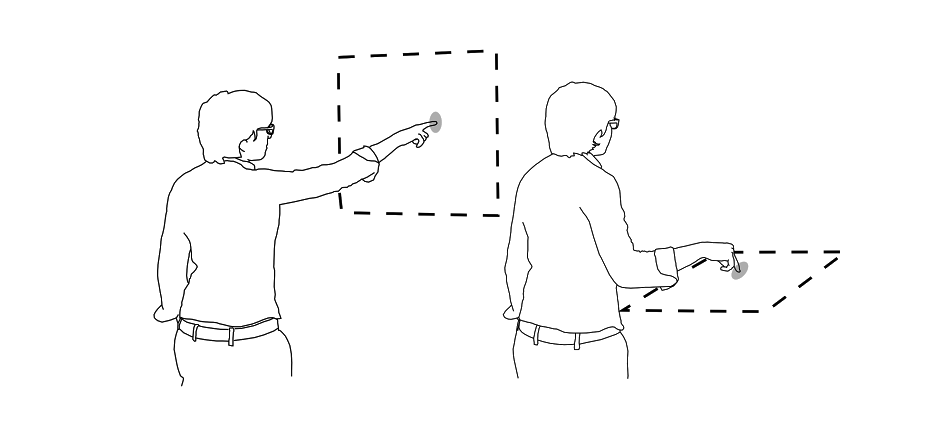
\includegraphics[scale=0.3]{image/touch.png}
	\caption{Représentation de l'espace d'interaction virtuel}
\end{figure}

Dans cet espace, il faut traquer la position de la main de l’utilisateur pour pouvoir mettre à jour la position de la souris et permettre la reconnaissance de gestes afin de savoir quand supprimer l’espace d’interaction virtuel concerné.

\begin{figure}[!ht]
	\center	
	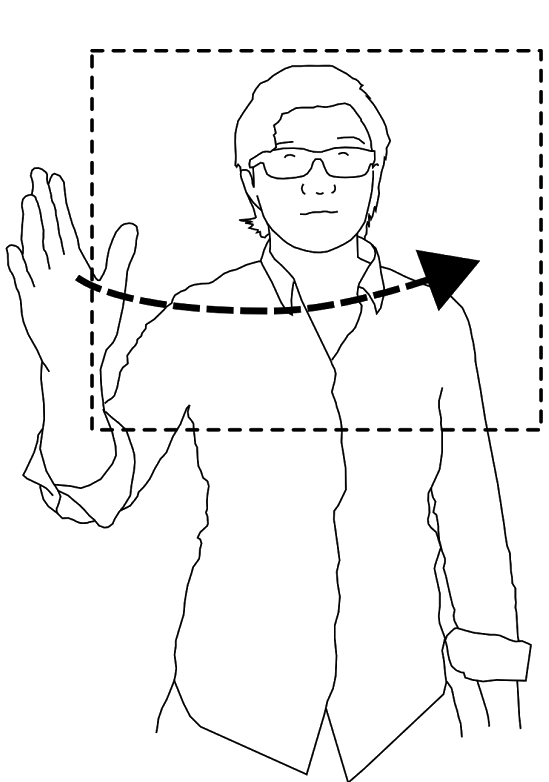
\includegraphics[scale=0.2]{image/remove.png}
	\caption{Suppression de l'espace d'interaction virtuel}
\end{figure}
	
\newpage

\section{Kinect}

La Kinect est un outil développé par l'entreprise PrimeSense et popularisé par Microsoft avec la Xbox 360, qui l’utilise comme un periphérique de jeu permettant de jouer sans manette. Ce dispositif possède une caméra couleur ainsi qu’une caméra et un émetteur infrarouge. L’émetteur envoie des rayons infrarouges structurés ce qui permet, à l’aide de la caméra infrarouge, d’obtenir des informations sur la profondeur de l’image acquise en analysant la projection des points. 

\begin{figure}[!ht]
	\center	
	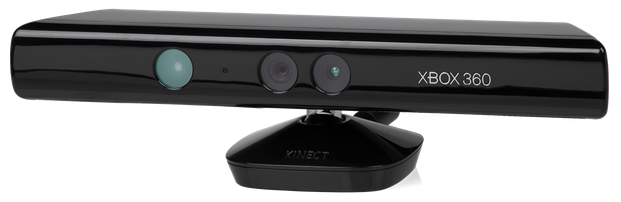
\includegraphics[scale=0.5]{image/kinect.png}
	\caption{La Kinect}
\end{figure}

Grâce à ces images, nous pouvons obtenir des données sur la position dans un environnement en 3D des différents membres des utilisateurs et donc de reconnaitre les mouvements effectués par l’utilisateur. 

La caméra Kinect possède un taux d'acquisition de 30 images par seconde avec une résolution de 640x480 pixels. Le capteur capte avec une portée minimale de 0.5 mètre et peut acquérir des objets situés jusqu’à 3.5 mètres dans un champ de vision horizontal de 57° et de 43° en vertical.

L'ajout du contrôle via Kinect est pertinent puisqu'il s'agit d'un outil grand public et à faible coût, contrairement a des solutions plus performantes, comme les ARTrack, qui ont un coût élevés et qui demande une calibration ainsi qu’un équipement des utilisateurs avec les dispositifs nécessaires.

Dans le cas de notre projet, la Kinect est utilisée pour tracker les personnes et plus particulièrement la position et l’orientation de leurs mains. Ces données sont envoyées via un serveur TUIO modifié. Pour que la Kinect soit plus performante le 1€ filter \cite{oneeuro} est utilisé pour supprimer le bruit et d’obtenir un pointeur virtuel plus stable. 



\section{Problématiques}

\subsection{Visualisation de l’espace virtuel}

Le problème qui se pose avec l’utilisation de l’espace virtuel est l’absence de retour visuel pour l’utilisateur ainsi que le manque de retour physique indiquant une action effectué. Dans notre cas nous avons un retour visuel car nous travaillons sur un prototype. Cependant, dans le cadre d’une utilisation grand public, l’utilisateur n’aura plus ce retour visuel. Il ne pourra pas avoir d’information sur l’emplacement de l’espace virtuel ni de la position de sa main par rapport à celui-ci.

\begin{figure}[!ht]
	\center	
	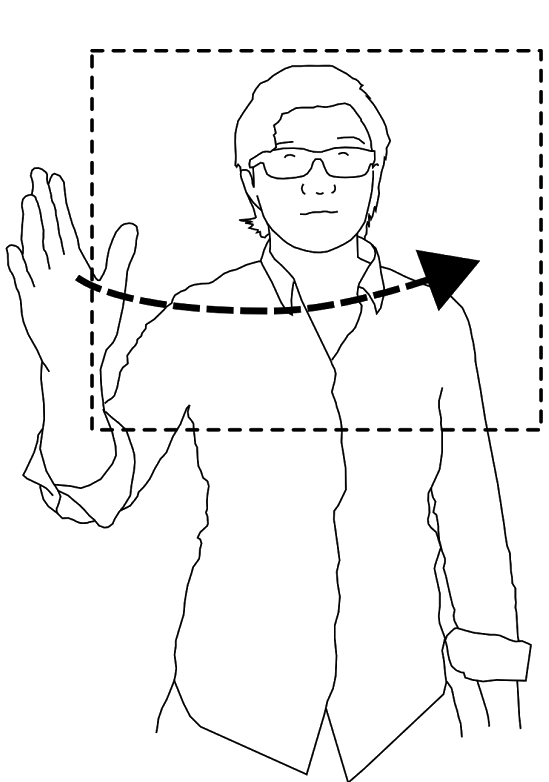
\includegraphics[scale=0.2]{image/remove.png}
	\caption{Visualisation de l'espace d'interaction virtuel}
\end{figure}

Ce manque d’information est troublant à l’utilisation. De plus lors d’une utilisation en multi-utilisateur, l’action de transmettre l’espace virtuel ou simplement de le localiser est complexe voir impossible. (citer article) La possibilité de pouvoir attacher un espace à un objet physique permettrait de résoudre ce problème de visualisation.


\subsection{Occlusion de la main par le support physique}

Dans le cas ou on utiliserait un support physique, plusieurs questions se posent sur l’occlusion. 
Le support peut dans certaines orientations empêcher le tracking de la main de l’utilisateur. Pour pallier à ce problème il faut, soit demander à l’utilisateur de tenir le support à plat face à la kinect, ce qui n’est pas confortable, ou placer plusieurs Kinect.
L’ajout de Kinects, ou de webcams supplémentaires peut nous permettre de visualiser la scène sous plusieurs angles et donc de suivre la main même quand celle-ci n’est pas visible par la Kinect principale.  

\subsection{Partage de l’objet virtuel}

Comme cité précédemment, le dernier problème est la difficulté pour partager l’objet virtuel. En effet, l’utilisateur courant doit sortir de l’espace virtuel puis le deuxième utilisateur doit rentrer dans cet espace pour effectuer le partage ce qui suppose que le deuxième utilisateur arrive à situer parfaitement l’espace virtuel dans le monde réel. Avec un support physique, il suffirait de partager le support pour partager l’espace virtuel par la même occasion.  
